\documentclass{article}
\usepackage[usenames]{color} %used for font color
\usepackage{amssymb} %maths
\usepackage{amsmath} %maths
\usepackage[utf8]{inputenc} %useful to type directly diacritic characters
%\usepackage[linesnumbered,ruled,vlined]{algorithm2e}
\addtolength{\topmargin}{-.975in}
%\pagenumbering{gobble}
\usepackage{url}
%\usepackage{hyperref}
\usepackage{float}
\usepackage{pgfplots}
\usepackage{tikz}
\usepackage{graphicx}
\usepackage[french]{babel}




\title{Troisième Rapport INF6404A : Application et Architecture}
\author{
	Alexandre Mao\\
	David Johannès \\
	Fabien Berquez \\
	Philippe Troclet \\
	D\'{e}partement G\'{e}nie Informatique et G\'{e}nie Logiciel \\
	\'{E}cole Polytechnique de Montr\'{e}al, Qu\'{e}bec, Canada \\
	\texttt{alexandre.mao@polymtl.ca}\\
	\texttt{david.johannes@polymtl.ca}\\
	\texttt{fabien.berquez@polymtl.ca}   \\
	\texttt{philippe.troclet@polymtl.ca}   \\
}
\date{31 mai 2016}

\usepackage{natbib}
\usepackage{graphicx}

\begin{document}

\maketitle

\section{Introduction}
Le monde d’IoT représente par définition un système “intégré”, où les différents objets interagissent entre eux, sont
inter-connectés, à travers l’échange d’informations et de commandes (requête, demande). Ces objets ont une forte probabilité d’être hétérogènes en termes de niveau de sécurité, de privacité minimal garanti, de technologie, de protocole de communication, et de politique d’exécution. Le challenge est ainsi davantage lié au besoin d’avoir une structure horizontale capable de gérer les spécifications de sécurité et de privacité de manière unique et homogène. Ces spécifications auront besoin en effet d’être instanciées sur des “entités” et auront potentiellement des interfaces d’implémentation, de spécification et de communication différentes.
\\

Les caractéristiques de IoT comprennent donc un réseau à très grande échelle des objets, une grande hétérogénéité au niveau des dispositifs et du réseau, et un grand nombre d'événements générés spontanément par ces objets. Malheureusement, toutes ces caractéristiques feront du développement des diverses applications et des services une tâche très difficile. En général, le middleware peut faciliter un processus de développement en intégrant des dispositifs informatiques et de communication hétérogènes, et en soutenant l'interopérabilité au sein des diverses applications et services.

En effet, un middleware fait abstraction de la complexité du système ou du matériel, permettant au développeur d'applications de concentrer tous ses efforts sur la tâche à résoudre, sans la distraction des préoccupations orthogonales au niveau du système ou du matériel. Ces complexités peuvent être liées à des préoccupations de communication ou au calcul plus généralement. Un middleware fournit une couche logicielle entre les applications, le système d'exploitation, les couches de communication réseau et les différents dispositifs du système, ce qui facilite et coordonne certains aspects du traitement coopératif. Du point de vue informatique, un middleware fournit une couche entre les logiciels d'application et des logiciels système. Dans l'IoT, l’hétérogénéité des dispositifs implique très souvent une hétérogénéité considérable dans les technologies de communication utilisées, ainsi que dans les technologies au niveau du système, c’est pourquoi un middleware devrait supporter ces deux types d’hétérogénéité. Nous avons donc besoin d’un middleware qui respecte des caractéristiques, que nous décrirons par des modules. Ces modules seront divisés en trois groupes : les modules fonctionnels, liés aux services et aux fonctions que notre middleware doit fournir ; les modules non-fonctionnels, liés à la Quality of Service (QoS), aux performances et aux différentes exigences que notre middleware devra prendre en compte; et les modules architecturaux, liés à l’architecture de notre middleware.
\\
\begin{figure}[h!]
	\hspace*{-1cm}
	\centering
	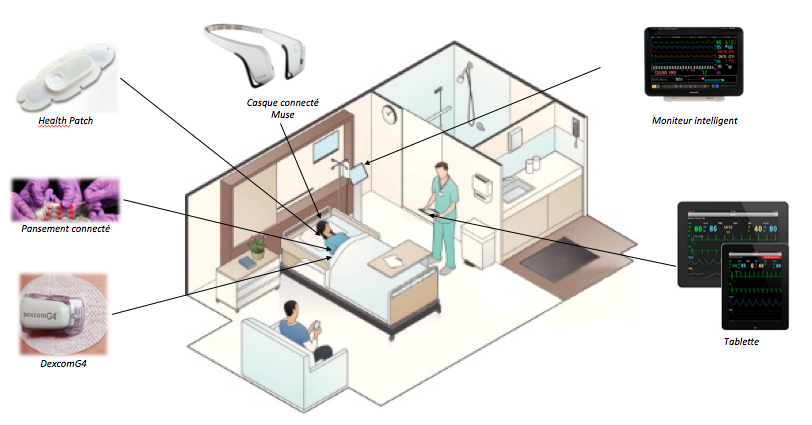
\includegraphics[width=1.1\textwidth]{Figure1.png}
	\caption{Couches Dispositifs, et Protocoles de Réseau et de Communication de notre Système}
	\label{fig:couches}
\end{figure}

Rappelons que notre sujet consiste à établir un système IoT dans le domaine Smart Health, et plus précisément dans les services de
soins intensifs des hôpitaux, afin de résoudre le problèmes de congestion et de surveillance en continu dans ces services. La Figure
\ref{fig:couches} nous permet de visualiser les choix de dispositifs et de protocoles de communication et de réseau que nous avons établis
dans le rapport précédent. Avant de commencer à décrire les différents modules dont nous aurons besoin dans notre middleware, ce que nous feront dans les section 2, 3, et 4, il est important de préciser le choix que nous avons fait concernant l’architecture générale de notre middleware. En effet, nous avons décidé de diviser notre middleware en deux couches différentes, la première étant liée au moniteur qui centralise toutes les informations des divers dispositifs présents dans la chambre du patient, et qui donc va gérer l’hétérogénéité entre les dispositifs présents dans l’environnement du patient. La seconde couche middleware est liée au Gateway de notre système, qui s’occupe de centraliser les informations de tous les moniteurs (le problème d’hétérogénéité se pose moins ici), et qui va faire le lien entre la couche de stockage et celle de liaison à la couche physique. Cette seconde couche va être celle qui permettra d’identifier les différents groupements de dispositifs à travers la connaissance des différents moniteurs intelligents.

La Figure \ref{fig:vueglobale} nous permet de visualiser la structure de notre système en considérant seulement les couches dispositifs, réseaux et communication, middleware, et architecture. Ainsi, dans les trois prochaines sections, notre tâche ne sera pas seulement de décrire les différents modules dont nous avons besoin dans notre middleware, mais aussi de décrire dans quelle(s) couche(s) middleware nous en avons besoin (possiblement les deux).

\begin{figure}[h!]
	\hspace*{-2.5cm}
	\centering
	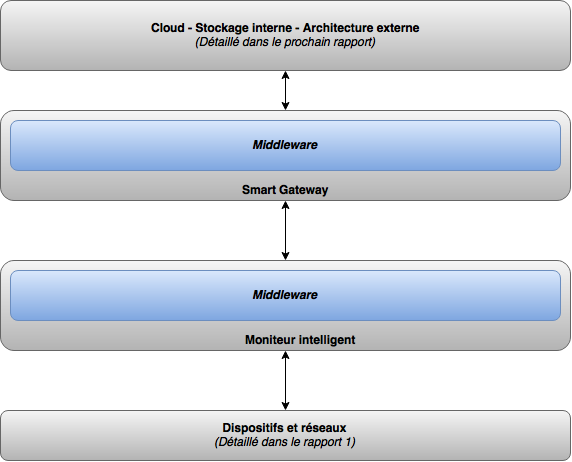
\includegraphics[width=1.4\textwidth]{Figure2.png}
	\caption{Vue Globale de notre Middleware au sein de notre Système}
	\label{fig:vueglobale}
\end{figure}


 
\section{Couche Applicative}
Dans cette section, nous présentons les différents services liés à notre solution. Pour se faire, nous regarderons et analyserons les différentes fonctionnalités de notre application à travers différents points de vue : celui du personnel médical (médecins et infirmiers), celui du personnel de la maintenance, celui de l'hôpital (en terme de gestion des ressources et des informations), celui de l'architecture (c'est-à-dire notre point de vue), et enfin celui des proches du patient.

\subsection{Du point de vue du Personnel Médical}
L’architecture que nous avons proposée et les différents capteurs qui pourront être mis en place ont pour but d’aider le personnel médical dans le suivi de l’état de santé du patient. Nous allons détailler ici les différents services fournis à travers des applications destinées au personnel médical de l’hôpital. Ces différents services sont consultables sur la figure \ref{medical}.
\\
\begin{figure}[h!]
	\hspace*{-2.5cm}
	\centering
	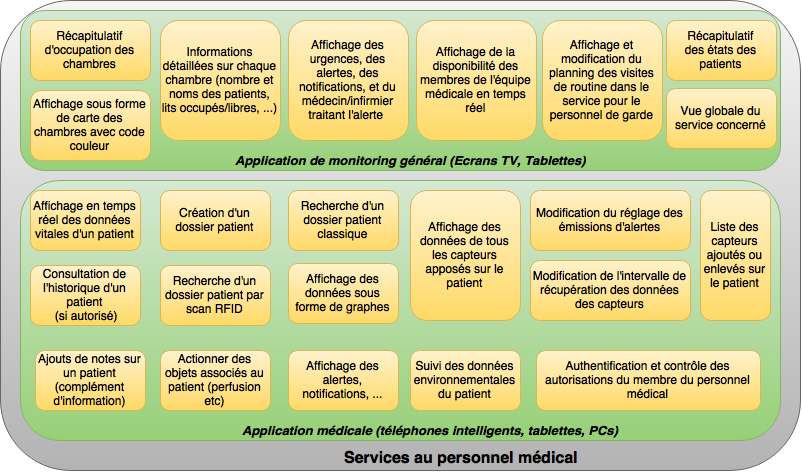
\includegraphics[width=1.4\textwidth]{medical.png}
	\caption{Services de la Couche Applicative du côté du Personnel Médical}
	\label{medical}
\end{figure}

Nous allons distinguer deux applications, l’une générale destinée au suivi des patients et du département de soins intensifs et la seconde application qui permettra un suivi plus poussé du profil d’un patient en particulier. La figure \ref{appli} illustre cette différenciation de services proposés en fonction de l'authentification. Nous allons détailler les différentes fonctionnalités de la première application destinée au suivi général des patients du département. En effet, nous pouvons supposer qu’au niveau du département de soins intensifs, il y a la présence d’une zone réservée au personnel d’astreinte, cette première application aura pour but d’aider le personnel médical dans la surveillance des patients, et va donc permettre de centraliser certaines des différentes informations récupérées des différents capteurs et des serveurs privés de l’hôpital. Cette première application sera destinée à un affichage sur des tablettes ou des écrans de télévision. 
\\
\begin{figure}[h!]
	\hspace*{-2.5cm}
	\centering
	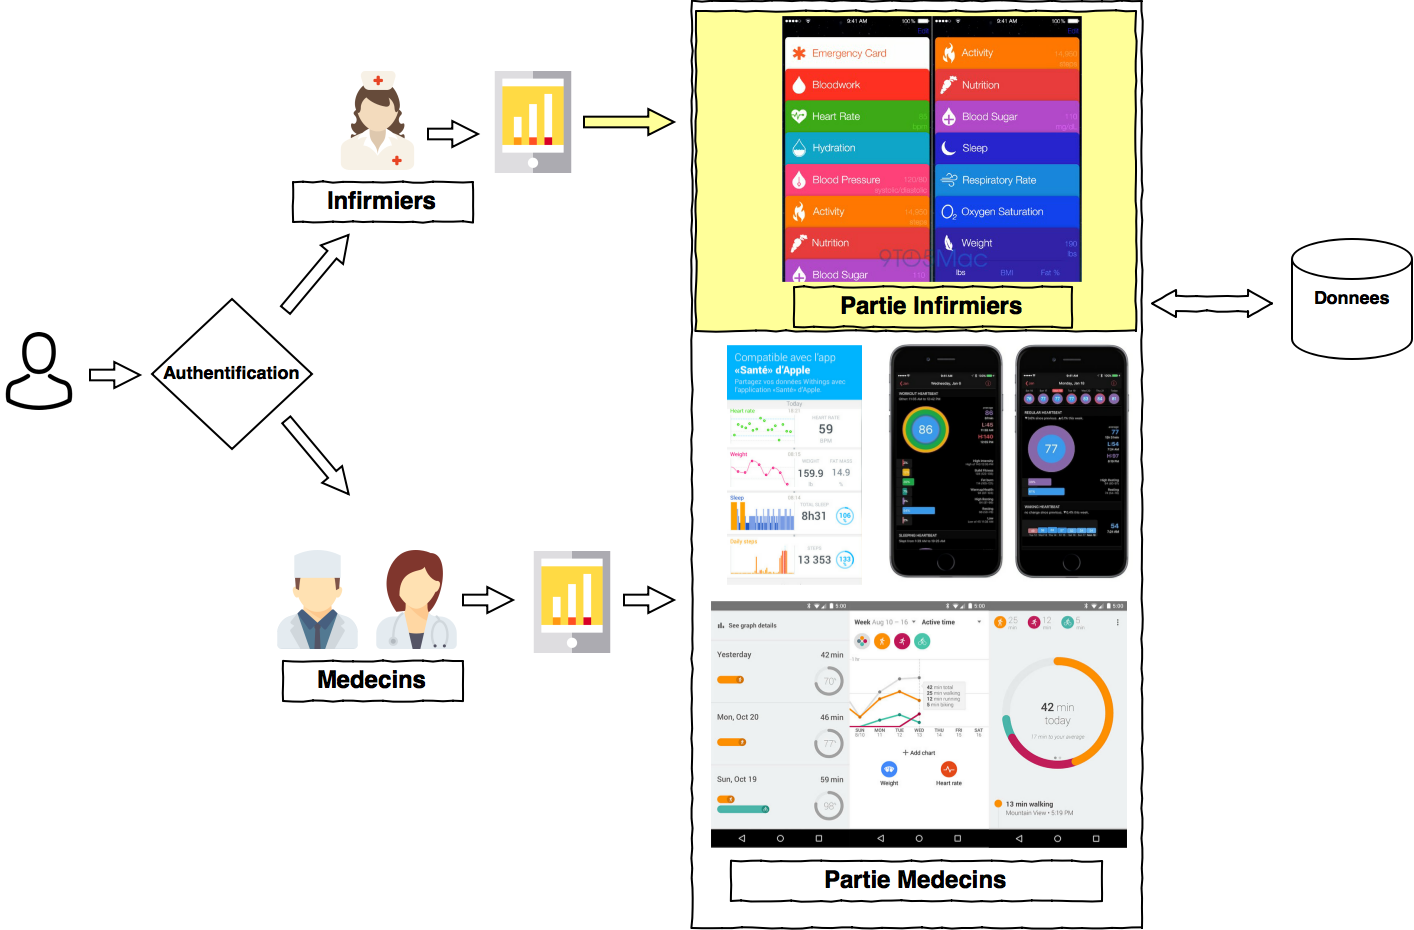
\includegraphics[width=1.4\textwidth]{Application.png}
	\caption{Différenciation des Services en fonction de l'Authentification du Personnel Médical}
	\label{appli}
\end{figure}

Pour intégrer les exigences de sécurité et de confidentialité que requiert le domaine médical, l’application contiendra un module
d’authentification qui assurera l’accès restreint aux données. Une fois l’authentification faite, l’application pourra être
utilisée de manière continue s’il n’y a pas de déconnexion ou d’interruption.


Une fois cette phase d’authentification faite, le ou les utilisateurs pourront accéder aux différentes données fournies par l’application provenant des capteurs et du Cloud. Par exemple, l’utilisateur pourra avoir accès aux différentes chambres, en sachant lesquelles sont occupées et lesquelles ne le sont pas.


L’application possédera ainsi une vue globale sur le département, avec la modélisation de l’occupation des chambres, l’état des différents patients présents dans le département de soins intensifs, et les informations générales permettant la surveillance du département.

Cette application aura la possibilité d’accéder à une page de consultation plus détaillée avec par exemple la possibilité d’avoir une vue sous forme de carte, sur laquelle un code couleur sera mis en place pour différencier, les chambres occupées des chambres libres. L’application permettra d’accéder à des informations plus précises sur les chambres, avec la possibilité de connaître l’occupation des chambres, le nom des patients présents, les lits occupés ou libres. Et l’une des fonctionnalités principales de l’application sera la notification des alertes avec l’affichage des différents lits et chambres qui auraient émis une notification, une alerte ou une urgence. Lors de la réception d’une urgence ou d’un alerte, l’application affiche en plein écran la chambre et le lit d’où provient l’alerte. S’il y a plusieurs alertes qui sont émises, l’application fera alors un affichage sous forme d’une division de l’écran avec la présence d’une file pour pouvoir afficher toutes les alertes selon le niveau et l’ancienneté. Pour chaque alerte, lorsqu’un médecin confirme la prise en charge de l’urgence, l’affichage se complète pour signaler la mise à jour de la situation au reste du personnel médical.

Le personnel médical peut être informé en temps réel de la disponibilité et de l’activité de leur collègue. Cela permettra au chef de secteur de mieux organiser les ressources humaines à sa disposition et ainsi optimiser le traitement des patients.

Le personnel médical d’astreinte aura accès a une page de consultation des prochaines visites à faire avec les informations nécessaires au bon déroulement de ces visites de routines (affichage du numéro des chambres, du nom des patients,), l’application sera reliée au système de planification de l’hôpital. Il y a aura donc la possibilité d’accéder à un planning pour ajouter, modifier, supprimer des visites à faire pour les différents patients.
\\

La seconde application aura pour but d’aider le personnel médical à faire un suivi de manière plus précise d’un patient.

Pour intégrer les exigences de sécurité et de confidentialité que requiert le domaine médical, l’application contiendra aussi un module d’authentification qui assurera l’accès restreint aux données. Une fois l’authentification faite, l’application accédera au profil de l’utilisateur connecté pour connaître les droits que possède cette personne et afficher les différentes possibilités de navigation selon les droits qui ont été trouvés.

Une fois l’utilisateur authentifié, il pourra accéder aux différentes données fournies par l’application provenant des capteurs et du Cloud. Les différentes données fournies par les capteurs placés sur le patient sont accessibles en temps réel, notamment pour tout ce qui est suivi des signes vitaux, et au besoin l’application peut, si les droits de l’utilisateur le permettent, accéder au historiques des différentes données du patient.

L’utilisateur pourra ajouter un dossier patient, pour cela il lui suffira de rentrer certaines informations précises et définies en concordance avec les besoins du personnel médical. L’accès au profil utilisateur sera facilite par la présence des puces RFID d’identification des patients près du lit et dans le bracelet de celui-ci. Il suffira alors d’un simple scan d’une des deux puces. La recherche classique d’un profil du patient sera toujours possible selon différents critères. Une fois le profil affiché, les informations sur le patient sont consultables, et selon les informations dont le membre du personnel médical aurait besoin, il pourra naviguer de façon à voir les informations générales sur le patient ou des informations plus détaillées.

Au niveau des différentes informations auxquelles aura accès l’utilisateur, nous pouvons voir les différents éléments suivant qui
proviennent des différents capteurs qui ont été proposés pour notre système. Il y a tout d’abord la possibilité d’accéder à
différentes informations vitales du patient comme le rythme cardiaque, la fréquence respiratoire, le rythme cardiaque, la
température du corps et la pression sanguine. Ces informations seront accessibles sous formes de graphes pour le suivi de l’état
de santé du patient. Les données des différents capteurs seront visibles à travers l’application, comme les données provenant du capteur pour la surveillance du cancer, ce qui permettra un suivi de l’évolution des différents indicateurs pour aider le diagnostic et le suivi du médecin, un accès au taux de glycémie du patient et son évolution, qui permettra ainsi au personnel médical d’injecter les bonnes doses d’insuline et permettre un suivi plus poussé de l’évolution de la glycémie, le suivi de l’activité cérébrale du patient sera aussi présent.

Le suivi de l’évolution des plaies sera aussi disponible grâce aux éventuels pansements intelligents mis en place sur le patient.
Le poids du patient pourra être surveiller, cet élément qui est un indicateur non vital, pourra permettre au personnel médical
d’avoir des renseignements supplémentaires quant à l’évolution de la santé du patient. Les mouvements des patients pourront être
suivis pour voir, notamment durant la phase de guérison, si le patient respecte bien ce qui a été indiqué par le personnel
médical. Par exemple, dans le cas où le patient doit restreindre ces mouvements, le personnel médical pourra savoir si ces
recommandations ont bien été suivies. Enfin les différentes données environnementales pourront être suivies pour notamment rassurer
les proches de la famille.

Aux différentes possibilités de consultation que l’utilisateur aura, s’ajoutera différentiations possibles sur les différents
éléments de l’environnement du patient. Il y aura la possibilité de modifier des paramètres de traitement des données sur le
patient, comme la possibilité de changer le temps d’émission des alertes, l’intervalle de temps entre la récupération de certaines
données depuis les capteurs, pour que le suivi puisse être vraiment propre à chacun des patients. Les paramètres de
traitement des données sur le patient et d’émission des alertes pourront être personnalisés pour pouvoir changer le temps
d’émission des alertes, l’intervalle de temps entre la récupération des données depuis les capteurs, le seuil d’émission des
alertes pour que le suivi soit le plus adapté possible au patient. L’application sera notifiée directement la mise en place ou le
retrait d’un nouveau dispositif par le personnel médical. 

Certains systèmes pourraient être directement contrôlés depuis l’application, comme le débit de la perfusion qui pourra être réglé à distance courte par le personnel médical. Pour ces fonctionnalités, une certaine sécurité sera mise en place en empêchant la modification si le membre du personnel médical n’est pas présent dans la pièce.

Les médecins et infirmiers pourront ajouter des notes au dossier du patient grâce à une fenêtre facilement accessible pour avoir un historique du suivi de l’état de santé du patient.

Cette application va permettre à l’utilisateur de recevoir les notifications d’alertes émises par les différents capteurs de
surveillance. Une fois que le médecin le plus adapté pour la gestion de l’alerte sera identifié par le système, un message sera
envoyé à travers le système pour le notifier  qu’une situation d’urgence a besoin de sa présence. Le médecin pourra alors notifier
de la prise en charge ou non de cette situation ce qui avertira le reste du personnel médical et permettra une meilleure gestion des ressources humaines du département.

\subsection{Du point de vue de la Maintenance}
Un hôpital doit avoir un équipement le plus fiable possible. En effet, une simple défaillance peut causer la mort du patient, ou
à défaut de graves dommages. Il est donc important de choisir prudemment les équipements à utiliser. Malheureusement l'équipement
sans faille n'existe pas et lorsqu'une panne se produit, il est capital de pouvoir déterminer l'origine de la défaillance. Pour
cela la présence de logs est indispensable à tous les niveaux. 
\newline

Au niveau du moniteur, il faut pouvoir savoir quel type de capteur s'est connecté (marque, modèle) afin d'identifier d'éventuelles
incompatibilités. Il faut également enregistrer les moments où le moniteur a donné un ordre, ainsi que son contenu.
Les réponses reçues sont aussi à conserver.
\newline

La passerelle intelligente (parfois appelée smart gateway) doit également avoir un historique des messages/demandes qu'elle a
reçus. Allié avec les logs issus d'un moniteur cela peut permettre d'identifier des problèmes réseaux, des interblocages et bien
d'autres dysfonctionnements.
\newline 

Pour des raisons similaires, des logs doivent être aussi présents au niveau du stockage interne et du cloud. En plus de permettre
une meilleure compréhension des pannes, ils pourraient avoir des applications au niveau de la sécurité. Entre autre, ils seraient
un moyen simple pour s'assurer que personne n'a essayé d'accéder à données qui ne leur sont pas destinées.
\newline

La présence de logs, impose de pouvoir les gérer. En effet, ces logs risquent d'être volumineux, il faut donc avoir la
possibilité de trier ces derniers afin de ne récupérer que les données pertinentes. Mettons que l'on ait l'intégralité des logs
d'une passerelle intelligente, il serait souhaitable de pouvoir extraire toutes les données relatives à un moniteur. De ce fait,
il faut intégrer un module de récupération de données permettant de filtrer les données via une description de ce que l'on veut
récupérer. Idéalement et afin d'être le plus flexible possible, ces descriptions seraient faites via un langage de requêtes
structurées. En effet, les données et capteurs utilisés peuvent varier d'un patient à l'autre, aussi lors de l'enquête suite à une
panne ou lors de tests, il est important faire du cas par cas et ne pas être prisonnier d'outils trop généraux.
\newline

Par ailleurs, la récupération de ses logs doit se faire de manière distincte de l'obtention des données d'un patient. Ces logs
étant destinés au service technique, aucune information personnelle ne doit transparaître. En particulier, ni le nom ni l'id du
patient ne doivent être visibles. De plus, le service technique doit savoir quelle version de chaque logiciel est présent sur
chaque objet connecté de l'hôpital. Cela permettrait d'agir efficacement si un bug, problème de compatibilité, etc ... Venait à se
produire.
\newline

Enfin, le système doit avoir un module consacré aux tests. Les équipements (moniteurs, passerelles) ont un rôle capital et une
défaillance de leur part aurait de graves conséquences. Aussi, le système doit faciliter la conception et mise en place de tests.
Pour cela, notre plateforme doit comporter un mode \textit{test} qui permettrait au technicien de suivre les données qu'il envoie.
Ce mécanisme permettrait la vérification de l'acheminement des données et que des décisions appropriées sont prises au regard de
ces dernières. Ce mode devra également permettre plus de contrôle: si une donnée de test relative à un taux de glucose trop élevé
est envoyée, il ne faut pas que le personnel médical soit dérangé car il s'agit de données fictives. Mais afin de vérifier
l'émission d'alerte, il est préférable que le technicien puisse préciser où l'alerte sera envoyée (probablement sur l'une des
machines dédiées aux tests que le service technique a en sa possession). Un autre requis de ce système est une dissociation entre
le mode test (ses données, ses décisions) et le fonctionnement du mode normal. Ces deux modes vont sûrement se côtoyer, mais il
est impensable que l'un interfère avec l'autre. Si les données venaient à se mélanger, cela pourrait être dangereux pour le
patient : un médecin pourrait prendre des décision basées sur des données fictives (destinées aux tests). De plus, si le service
technique venait à avoir accès à des données d'un patient (suit à un mélange entre les deux types de données), cela
représenterait une atteinte à la vie privée. Et il faut garantir que les réglages faits pour les tests ne se propage pas en dehors
du domaine de test, sinon le bien être et la santé des patients est à risque.

\subsection{Du point de vue de l'Hôpital}
La gestion des ressources est une discipline présente dans tous les domaines. Le domaine médical ne fait pas exception à cette
règle. En effet, un certain équipement est nécessaire pour traiter les malades. Ce matériel peut se dégrader avec le temps ou
suite à un accident. A terme il faudra donc le remplacer. Afin de procéder aux achats, il est préférable de faire un inventaire,
cela permet de faire des commandes globales et donc d'économiser de l'argent. De nombreux commerces ferment durant un inventaire
afin de simplifier l'opération, toutefois cette solution n'est pas envisageable dans le cas des hôpitaux en général, en
particulier cela serait inacceptable dans le service des urgences.  
\newline

Le système doit donc permettre de faire un inventaire. Il serait préférable qu'il permette non seulement de connaître le nombre de
dispositifs selon le type de ces derniers, mais aussi le nombre de dispositifs d'un certain modèle. En effet, un modèle pourrait
posséder plus de fonctionnalités, ce qui le rendrait indispensable pour certaines situations, ou du moins plus pratique. Intégrer
cette fonctionnalité à notre système plutôt que de se basé sur un logiciel/mécanisme déjà existant a quelques avantages non
négligeables. En particulier, sous l'hypothèse que chaque capteur possède un trait unique, il est possible d'automatiser une
partie du processus. Comme exemple de trait distinctif, on peut penser aux adresses mac que des constructeurs donnent à leurs
produits. Le principe de fonctionnement serait le suivant: lorsque le capteur se déclare à son moniteur, ce dernier informerait le
système (via un message à la passerelle intelligente) de la connexion qui vient de s'établir. La passerelle pourrait alors
informer un serveur interne qu'un capteur ayant un tel id vient d'initier une connexion. Le système vérifie s'il connaît cet id,
si ce n'est pas le cas il envoie un message à la passerelle demandant plus d'information. Il sera alors de la responsabilité de la
passerelle de le renseigner.  
\newline

Par ailleurs,en plus de connaître le nombre d'appareils, il peut être utile de pouvoir tracer des courbes récapitulant
l'utilisation par type d'appareil. En effet, la possibilité de calculer diverses statistiques permettrait de mieux anticiper les
besoins. En outre, cela est indispensable pour la prise de décision. En l'absence de telles statistiques, il est difficile de
décider le nombre d'appareils à acheter.  
\newline

En plus de pouvoir gérer les ressources, l'hôpital doit également gérer les patients. L'administration doit pouvoir créer un
nouveau dossier pour le patient ou ouvrir un dossier existant. Les informations présentes dans ces dossiers doivent pouvoir être
modifiées, complétées et sauvegardées. Certaines informations perdent de la valeur avec le temps, connaître la température dans
une chambre il y un an a peu d'intérêt. De même connaître l'intégralité des relevés cardiaques un an après n'est pas pertinent.En
plus de pouvoir supprimer des informations manuellement, il est nécessaire de pouvoir le faire de manière automatique pour
certaines données. De plus, conserver un dossier trop longtemps n'est pas nécessairement utile. Il est donc souhaitable que au
bout d'un certain temps ceux-ci soient supprimés automatiquement. Cela permettrait d'éviter la saturation de l'espace de stockage.
\newline

Par ailleurs, un système de gestion de paiement serait utile. Retenir le numéro de sécurité sociale, l'identifiant de la mutuelle
du patient et le statut de paiement serait particulièrement utile. Dans le premier cas, cela permettrait de facturer directement
les organismes payeurs sans avoir à déranger le patient ou la famille. Dans le second cas, cela permettrait de connaître les
patients ne s'étant pas acquittés de leur dû. Et de le leur rappeler si besoin est.
\newline

La présence d'un cloud (public ou privé) impose de pouvoir lire et écrire dessus. Le cloud privé servira de sauvegarde pour les
données du stockage interne. Il est donc important que ces données soient copiées à intervalles réguliers. Le cloud public, lui
contiendra des données anonymisées mises à disposition d'universités ou d'organismes de recherche pour mener à bien des études.
Ainsi que des informations peu sensibles destinées à la famille du patient. Ce cloud public sera également chargé de faire tourner
les différents programmes d'interaction destinés à la famille du patient.

Bien sûr, l'accès à ces fonctionnalités doit être surveillé et sécurisé. De manière grossière, on peut résumer les différentes
fonctionnalités du présent module de la manière suivante.
\begin{enumerate}
    \item gestion des informations dans le cloud
    \item gestion des informations stockées en interne
    \item gestion du cycle de vie des informations stockées
    \item sécurisation de l'accès aux données (que ce soit en lecture ou en écriture)
\end{enumerate}

\subsection{Du point de vue de l'Architecture}
Du point de vue architectural, à savoir de notre point de vue, le système que nous mettons en place au niveau de la couche applicative doit respecter plusieurs requis, notamment pour permettre à notre application d'être conforme aux normes juridiques du milieu médical. Les services prévus à cet effet apparaissent à la figure \ref{architecture}.
\\
\begin{figure}[h!]
	\hspace*{-2.5cm}
	\centering
	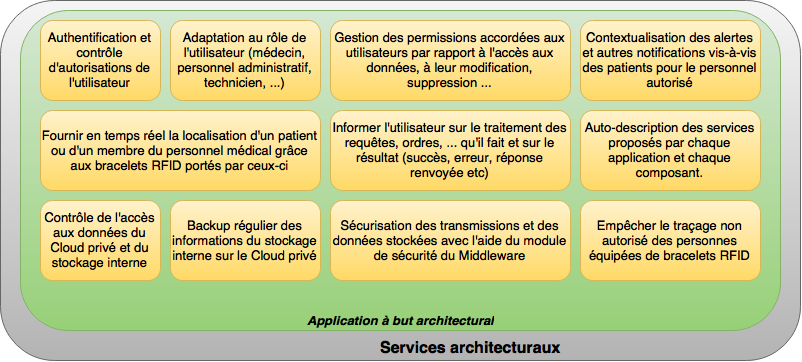
\includegraphics[width=1.4\textwidth]{architecture.png}
	\caption{Services de la Couche Applicative du côté de l'Architecture}
	\label{architecture}
\end{figure}

L'application proposée devra tout d'abord s’adapter, en terme de services proposés, à l’utilisateur, que ce soit le médecin, l'infirmier, la personne de la maintenance, le proche de la famille, ou l'hôpital. Ainsi, un système d’authentification est mis en place, et la personne devra s’identifier pour avoir accès aux services proposés. Chaque personne n’aura par conséquent pas les mêmes permissions, que ce soit en terme de visualisation des informations, mais aussi en terme de modifications de celles-ci. Ainsi, le médecin aura accès à l’historique des données et aux données courantes concernant le patient, et il pourra aussi apporter des modifications ; l’infirmier n’aura accès qu’aux données courantes ; la personne de la maintenance aura accès uniquement à l’historique des informations concernant les différents dispositifs utilisés ; l'hôpital aura accès à tout type d'informations et pourra les modifier afin de supprimer les informations périmées ou non utiles ; le proche de la famille pourra avoir accès aux informations non sensibles du patient afin d'avoir une connaissance de l'environnement du patient.

Au vu de ce qui a été dit précédemment, il faudra de l'interopérabilité à travers les différents services proposés, qui devront s'adapter à l'utilisateur.

Aussi, les informations et les permissions liées à celles-ci et fournies aux différents utilisateurs doivent dépendre de l’utilisateur. C'est pourquoi les permissions (modification, lecture, écriture) et les informations (log, informations liées aux patients) seront différentes selon l’utilisateur. L’application doit donc aussi restreindre les permissions concernant la modification ou la suppression des informations collectées, et cela en fonction de l'utilisateur.

Les informations liées au patient ne devront bien évidemment pas être anonymisées, mais au contraire contextualisées. En effet, si par exemple le médecin reçoit une alerte liée à un cas d'urgence, il faudra qu'il sache quel patient a généré cette alerte pour pouvoir le voir et gérer ce problème.

Notre système devra fournir la localisation des patients (grâce à leur puce RFID) qui est essentielle afin de savoir d'où provient une alerte ou une urgence (quel patient, et plus précisément quel capteur a généré telle information). La localisation du personnel médical (notamment grâce à la puce RFID des médecins) sera également fournie par le système, car elle est nécessaire pour attribuer une alerte ou une urgence à un personnel médical. Il faudra également gérer la localisation du personnel médical, car les déplacements générés par les médecins (et repérés par leur puce RFID) produisent des événements, et les services doivent s'adapter et prendre en considération ces événements (par exemple pour localiser le médecin le plus proche en cas d'urgence).

L’application devra fournir un feedback aux utilisateurs lorsque ceux-ci l'utilisent. Ce feedback servira à informer l’utilisateur que sa demande a été traitée, ou que l’indisponibilité du système n’a pas permis de traiter sa demande. Ce feedback devra être rapide dans le cas où les utilisateurs sont le personnel médical ou le personnel de maintenance (afin d'accélérer le traitement les alertes liées aux dispositifs ou au patient).

Les services proposés par l'application fourniront une auto-description, à savoir qu'ils donneront une description de ce qu'elles proposent (accès aux données, modification, historique, prise de rendez-vous, etc).

Comme indiqué précédemment dans le deuxième rapport, en plus d'un stockage interne, deux différents Cloud \cite{cloud} seront mis en place principalement pour le stockage des données. Le système intègrera tout d'abord un Cloud privé afin de stocker les informations sensibles et importantes, telles que les informations liées au patient et celles liées aux dispositifs et à leur état (les log). Ainsi, seuls les utilisateurs appartenant à l’hôpital (personnel médical, hôpital, personnel de maintenance) pourront y avoir accès. Le Cloud privé a la particularité par définition d'être isolé (car un seul et même serveur gère l’ensemble des données pour tous les utilisateurs), ce qui permet d'avoir une première protection et empêchera les attaques entre machines virtuelles (cross virtual machine attack). Étant donné que l'utilité du Cloud privé n'est liée qu'au stockage et à l'enregistrement (backup) d'informations, l'utilisateur n'aura tout simplement qu'à effectuer des requêtes pour avoir accès aux informations qu'il désire. C'est pourquoi l'utilisation du Cloud privé en tant que SaaS (Software as a Service) est suffisant, et l'application de gestion de données sera fournie par le fournisseur de ce Cloud.

Un Cloud public sera également utilisé au sein de notre système. Il stockera les informations non sensibles liées au patient et sera accessible par les proches du patient. Dans ce cas là, les données seront hébergées sur plusieurs serveurs eux-mêmes accessibles par un certain nombre d’utilisateurs, ce qui ne pose pas de problèmes ici car les informations stockées dans ce Cloud ne seront pas sensibles. Aussi, dans le Cloud public, en plus de l'application de gestion de données, nous fournirons une application d'authentification et de création de compte (pour permettre à chaque proche du patient d'avoir un compte), une application de rendez-vous (pour permettre aux proches du patient de prendre rendez-vous avec le médecin qui prend en charge le patient), et une application de messagerie instantanée (entre les proches du patient et le personnel médical). Comme nous fournirons dans ce Cloud l'application, nous aurons besoin d'un PaaS (Plateform as a Service).

Notre système devra automatiser le stockage des informations, depuis le stockage interne jusqu'au Cloud privé (avec un backup régulier, toutes les 6 heures par exemple) et public.

Afin de renforcer la sécurité et la confidentialité des informations (notamment celles liées au patient) dans les Cloud public et privé \cite{singh2015twenty}, il nous faudra crypter les informations stockées dans ces Cloud. L'accès aux informations liées au patient, au personnel médical et de maintenance, ainsi qu'aux ressources de l'hôpital (les dispositifs) devront être elles aussi sécurisées. C'est pourquoi toutes les communications vers les services proposés, vers les utilisateurs finaux, ainsi que toutes les communications provenant des services (et donc générées par les utilisateurs) devront être sécurisées. Comme dit précédemment, le Cloud privé servira aussi de backup (qui sera crypté), ce qui permettra une récupération sécurisée des informations en cas de problèmes. Afin de sécuriser et d'avoir un meilleur contrôle d'accès, et dans le cadre de l'authentification des utilisateurs, un identifiant unique sera fourni à chaque utilisateur. Notre système devra également rendre difficile l'espionnage de communication de messages à travers nos services, et devra empêcher le traçage des utilisateurs qui possèdent une puce RFID (médecin et patient) par des entités non autorisées, toujours pour améliorer la sécurité et la confidentialité. 

Enfin, notre système devra toujours permettre à un service d'être accessible par un utilisateur qui a le droit d'y accéder (pour assurer la disponibilité de notre application), et les informations qui circulent dans notre système devront être fiables, surtout en ce qui concerne les informations sensibles (qui peuvent potentiellement générées des alertes et des urgences liées au patient ou au dysfonctionnement des dispositifs).

\subsection{Du point de vue des Proches du Patient}
Le système que nous proposons dans le présent document possédera des services accessibles depuis l'extérieur, et que nous pouvons visualiser à la figure \ref{famille}. Parmi ces
fonctionnalités, certaines seront dédiées à la famille des patients. Ces services auraient, bien entendu, un contrôle d'accès très
strict. Une possibilité que nous avons envisagée est l'envoie d'un sms aux numéros à prévenir en cas d'urgence d'un patient. Ce
sms contiendrait un mot de passe et un identifiant valides que durant la période d'hospitalisation. Le destinataire pourrait alors
se connecter à un site web (via une connexion sécurisée) où il pourrait trouver différentes informations et différents conseils. 
De plus, dans le but de partager l'information avec des proches non présents sur la liste des personnes à contacter en cas d'urgence
, les personnes contactées par l'hôpital pourraient initier une procédure de création de compte pour d'autres proches. En revanche,
les comptes créés de cette manière ne pourraient pas créer d'autres comptes à leur tour. Ce mécanisme permettrait un meilleur contrôle
sur la création de comptes. On suppose que les proches à prévenir en cas d'urgence sont dignes de confiance, et que de ce fait
il n'y aura pas de création non légitimes de comptes.
\newline
\begin{figure}[h!]
	\hspace*{-2.5cm}
	\centering
	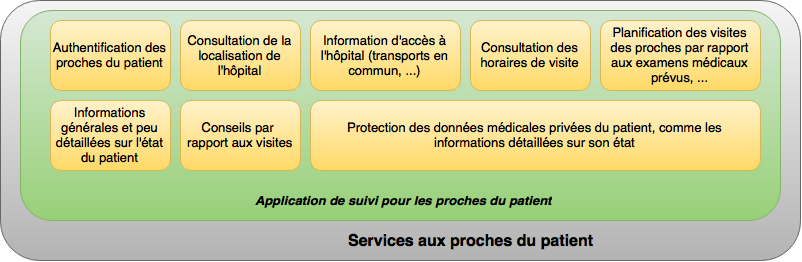
\includegraphics[width=1.4\textwidth]{famille.png}
	\caption{Services de la Couche Applicative du côté des Proches du Patient}
	\label{famille}
\end{figure}

Les informations visibles seraient la localisation de l'hôpital, comment s'y rendre ainsi que la chambre du patient. On pourrait
ajouter à cela les horaires des visites. Si l'on désire pousser cette idée plus loin, on peut imaginer un système où la famille
pourrait prendre rendez-vous sur un calendrier. S'il y a trop de visiteurs sur la période choisie, la demande de visite sera
refusée et l'utilisateur sera invité à choisir un autre moment. Ce système permettrait de mieux étaler les visites, évitant ainsi
que le patient ait trop de visiteurs à un certain moment, et aucun à d'autres moments. Cela permettrait aussi d'éviter que des
visiteurs viennent à une période où une opération est prévue. Ce qui les obligerait à rebrousser chemin. En revanche, les
informations médicales sensibles du patient ne seraient pas affichées, d'une part pour éviter une certaine atteinte à la vie
privée, et d'autre part pour limiter les mouvements de panique du côté des utilisateurs. Toutefois les informations médicales
utiles à la famille seraient accessibles. Cela permet d'empêcher que le service téléphonique de l'hôpital soit  surchargé par des
appels de proches exigeant des nouvelles.De manière générale, les consignes à respecter lors d'une visite seraient visibles sur
ce site. Et certaines informations sans lien direct avec l'hôpital mais utiles pour le confort des patients pourraient être
ajoutées. Connaître l'adresse de l'hôtel (ou équivalent) le plus proche serait, par exemple, un plus pour les visiteurs.
\newline

En plus des informations citées plus haut, nous aurions également des conseils à l'intention des personnes qui rendent visite aux
patients. Ces conseils pourraient être personnalisés selon le patient. A titre d'exemple, si leur traitement leur interdit un certain type d'aliments
cela serait précisé. 
\newline

Pour conclure cette partie, on notera qu'un tel système permettrait de réduire la charge du service public de l'hôpital, car de
nombreuses responsabilités qui étaient auparavant à leur charge seraient maintenant remplies par le site internet. De plus, il permettrait
d'améliorer l'expérience du visiteur en lui fournissant des informations et services utiles et disponibles à toutes heures.
Précisons que ce service devrait tourner sur le cloud public de l'hôpital.
\newline

Les services présentés ne peuvent être efficaces en l'absence de certains requis, qu'il convient de présenter.
\begin{enumerate}
    \item disponible : une forte disponibilité n'est pas requise, mais si le site discuté plus haut n'est pas accessible alors les
    responsabilités qui assuraient seraient de nouveau à la charge du personnel.
    \item Fiable : pour les mêmes raisons que précédemment. De plus, il doit également être fiable dans le sens commun du terme.
    En effet, si les informations présentées ne sont pas véridiques, l'hôpital perd en crédibilité. Et il risque de subir la
    colère et l'inquiétude des proches.
    \item sécurité : les communications doivent commencer par une phase d'authentification et être toujours chiffrées.
 \end{enumerate}

\subsection{Récapitulatif}
TODO écrire une nouvelle intro
%---------------------Début ancienne intro---------------------
%--------------------------------------------------------------
%Le monde d’IoT représente par définition un système “intégré”, où les diffé\-rents objets interagissent entre eux, sont inter-connectés, à travers l’échange d’informations et de commandes (requête, demande). Ces objets ont une forte probabilité d’être hétérogènes en terme de niveau de sécurité, de privacité minimale garantie, de technologie, de protocole de communication, et de politique d’exécution. Le challenge est ainsi davantage lié au besoin d’avoir une structure horizontale capable de gérer les spécifications de sécurité et de privacité de manière unique et homogène. Ces spécifications auront besoin en effet d’être instanciées sur des “entités” et auront potentiellement des interfaces d’implémentation, de spécification et de communication différentes \cite{vermesan2014internet}.
%\\

%Les caractéristiques de IoT comprennent donc un réseau à très grande échelle des objets, une grande hétérogénéité au niveau des dispositifs et du réseau, et un grand nombre d'événements générés spontanément par ces objets. Malheureusement, toutes ces caractéristiques feront du développement des diverses applications et des services une tâche très difficile. En général, le middleware peut faciliter un processus de développement en intégrant des dispositifs informatiques et de communication hétérogènes, et en soutenant l'interopérabilité au sein des diverses applications et services.

%En effet, un middleware fait abstraction de la complexité du système ou du matériel, permettant au développeur d'applications de concentrer tous ses efforts sur la tâche à résoudre, sans la distraction des préoccupations orthogonales au niveau du système ou du matériel. Ces complexités peuvent être liées à des préoccupations de communication ou au calcul plus généralement. Un middleware fournit une couche logicielle entre les applications, le système d'exploitation, les couches de communication réseau et les différents dispositifs du système, ce qui facilite et coordonne certains aspects du traitement coopératif. Du point de vue informatique, un middleware fournit une couche entre les logiciels d'application et des logiciels système. Dans l'IoT, l’hétérogénéité des dispositifs implique très souvent une hétérogénéité considérable dans les technologies de communication utilisées, ainsi que dans les technologies au niveau du système, c’est pourquoi un middleware devrait supporter ces deux types d’hétérogénéité \cite{li2015iot}. Nous avons donc besoin d’un middleware, et plus précisément de modules au sein de ce middleware, qui respecte des caractéristiques, que nous décrirons par des exigences. Ces exigences seront divisées en trois groupes : les exigences fonctionnelles, liées aux services et aux fonctions que notre middleware doit fournir ; les exigences non-fonctionnelles, liées à la Quality of Service (QoS), aux performances et aux différents requis que notre middleware devra prendre en compte; et les exigences architecturales, liées à l’architecture de notre middleware. La description de ces exigences apparaît à la section 2.
%\\
%\begin{figure}[h!]
	%\hspace*{-1cm}
	%\centering
	%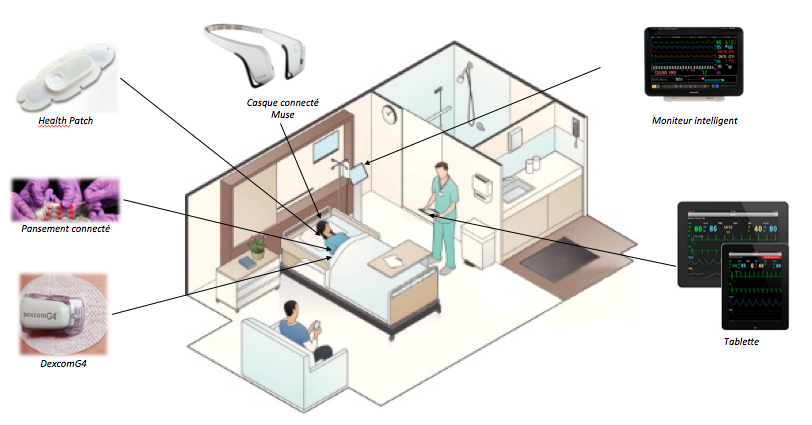
\includegraphics[width=1.1\textwidth]{Figure1.png}
	%\caption{Couches Dispositifs, et Protocoles de Réseau et de Communication de notre Système}
	%\label{fig:couches}
%\end{figure}

%Rappelons que notre sujet consiste à établir un système IoT dans le domaine Smart Health, et plus précisément dans les services de
%soins intensifs des hôpitaux, afin de résoudre le problèmes de congestion et de surveillance en continu dans ces services. La Figure
%\ref{fig:couches} nous permet de visualiser les choix de dispositifs et de protocoles de communication et de réseau que nous avons établis
%dans le rapport précédent. Avant de commencer à décrire les différents modules dont nous aurons besoin dans notre middleware, ce que nous feront dans la section 3, il est important de préciser le choix que nous avons fait concernant l’architecture générale de notre middleware. En effet, nous avons décidé de diviser notre middleware en deux couches différentes, la première étant liée au moniteur qui centralise toutes les informations des divers dispositifs présents dans la chambre du patient, et qui donc va gérer l’hétérogénéité entre les dispositifs présents dans l’environnement du patient. La seconde couche middleware est liée au Gateway de notre système, qui s’occupe de centraliser les informations de tous les moniteurs (le problème d’hétérogénéité se pose moins ici), et qui va faire le lien entre la couche de stockage et celle de liaison à la couche physique. Cette seconde couche va être celle qui permettra d’identifier les différents groupements de dispositifs à travers la connaissance des différents moniteurs intelligents.

%La Figure \ref{fig:vueglobale} nous permet de visualiser la structure de notre système en considérant seulement les couches dispositifs, réseaux et communication, middleware, et architecture. Ainsi, dans les prochaines sections, notre tâche ne sera pas seulement de décrire les différents modules dont nous avons besoin dans notre middleware, mais aussi de décrire dans quelle(s) couche(s) middleware nous en avons besoin (possiblement les deux).

%\begin{figure}[h!]
	%\hspace*{-2.5cm}
	%\centering
	%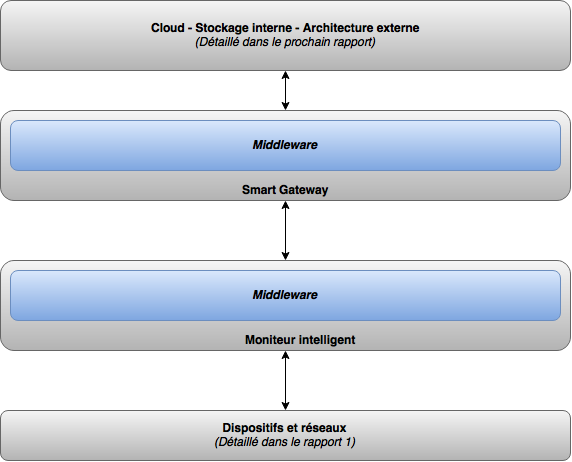
\includegraphics[width=1.4\textwidth]{Figure2.png}
	%\caption{Vue Globale de notre Middleware au sein de notre Système}
	%\label{fig:vueglobale}
%\end{figure}
%-------------------- Fin ancienne intro ----------------------
%--------------------------------------------------------------


\section{Sécurité et Confidentialité}
Dans cette section, nous discuterons de la sécurité et de la privacité au sein de notre système, à savoir à travers les différentes couches du système. Les modules de notre couche de sécurité et de protection de vie privée apparaissent à la figure \ref{securite}.
\newline
\begin{figure}[h!]
	\centering
	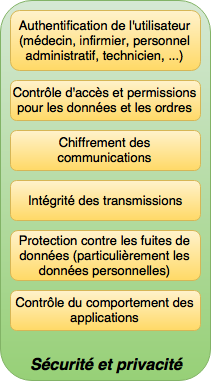
\includegraphics[width=0.5\textwidth]{securite.png}
	\caption{Couche Sécurité et Privacité de notre Solution}
	\label{securite}
\end{figure}

\subsection{Présentation de la problématique}

Dans les systèmes reposant sur l’Internet of Things, la sécurité et la protection de la vie privée sont de manière générale des problématiques majeures, à la fois car les données recueillies par les différents capteurs peuvent être intrusives et révéler énormément de choses sur une personne, et avoir ainsi des conséquences pour la vie de tous les jours, mais aussi car ces systèmes comprennent souvent des actionneurs ou des objets capables d’agir, dont les répercussions en cas de mauvaises utilisations ou d’utilisations détournées peuvent être nuisibles. Ainsi, la sécurisation des accès à ces actionneurs, aux sources des données, ainsi qu’à toute transmission ou système manipulant les données recueillies doit être particulièrement étudiée et soigneusement mise au point.

Dans notre système Smart Health, ces problématiques sont d’autant plus importantes de par le caractère vital et hautement personnel de ces données. La sécurité et la protection de la vie privée sont dans ce type de système fortement et étroitement liées tout en ayant certaines spécificités propres. Pour les problèmes de sécurité (d’un point de vue informatique), nous avons bien entendu la sécurisation des actionneurs quels qu’ils soient. Dans notre système, cela correspond par exemple à la sécurisation du dispositif contrôlant le débit des perfusions. Une personne mal intentionnée pourrait par exemple envoyer un ordre dangereux voire mortel. De même un dysfonctionnement non maîtrisé dans le système ou dans les capteurs aux alentours pourrait avoir des conséquences néfastes. C’est pourquoi nous avons dû prendre en compte cette problématique particulière. Nous verrons dans la suite de cette section les mesures que nous avons prises pour assurer la sécurité et la protection de la vie privée. A la fois concernant la vie privée et la sécurité, nous avons bien entendu dû nous assurer que les données médicales propres à chaque patient soient correctement retranscrites, cloisonnées et que seules les personnes autorisées aient accès à ces données.

\subsection{Prise en compte de cette problématique dans la couche physique}

Ces problématiques étant présentes tout au long du cycle d’utilisation du système, nous avons dû réfléchir sur chacune des couches à comment offrir un niveau optimal de sécurité et de protection de la vie privée. Notre solution détaillée dans les deux rapports précédents ainsi que dans celui-ci comprend un grand nombre d’éléments répondant à ces objectifs, que nous récapitulons ici.

Dans la couche physique et réseau, le travail essentiel à réaliser a été de trouver des mécanismes de sécurité applicables à des capteurs et dispositifs contraints en terme de ressources et de possibilité de calcul. Il était donc hors de question d’utiliser par exemple des mécanismes lourds de chiffrage des données. Nous avons donc opter pour l’utilisation de protocoles de communication réseau des couches basses comprenant déjà certains mécanismes intégrés de chiffrage des données, qui sont plus légers et pris en charge nativement par les implémentations des protocoles. Ainsi, nous avons retenu trois protocoles dont deux comprennent des mécanismes de chiffrage : IEEE 802.15.4 et Bluetooth Low Energy. Le troisième protocole choisi, RFID, nécessite d’une part une présence physique à proximité immédiate du lit et/ou du patient, et d’autre part l’accès au système central de l’hôpital pour que les informations soient utilisables. Ainsi, nous avons limité fortement les fuites possibles concernant la vie privée en reportant pour les protocoles non sécurisés la charge sur le middleware des moniteurs intelligents et de la passerelle, qui ont, eux, la capacité nécessaire à contrôler les accès aux données. De plus, Bluetooth Low Energy et IEEE 802.15.4 sont caractérisés par la nécessité d’apparier les dispositifs communicants, ce qui permet de contrôler davantage les dispositifs participant au réseau de capteurs autour du client. Enfin, les protocoles applicatifs choisis pour communiquer avec les capteurs, les actionneurs, les moniteurs intelligents, ou la passerelle, ou pour récupérer des informations depuis les capteurs permettent également l’utilisation de couches spécialisées dans la transmission sécurisée, comme DTLS ou TLS, ce qui renforce la protection offerte.
 
\subsection{Prise en compte de ces problématiques dans le middleware}

Si nous avons pris certaines précautions détaillées précédemment dans la couche physique, celles-ci se révèlent limitées par les capacités des appareils concernés. La deuxième couche, celle du middleware, est idéale pour implanter des services de sécurité plus avancés. C’est ce que nous avons choisi de faire de diverses manières. Le middleware que nous avons réalisé est en réalité distribué : une partie de ce middleware est déployé sur chacun des moniteurs intelligents qui constituent les sinks des réseaux de capteurs, et l’autre partie est présente sur la passerelle intelligente. La sécurité et la protection de la vie privée étant des problèmes transverses, le système de sécurité du middleware est présent sur chacune de ces parties.

Son premier rôle est l’authentification : pour chaque requête effectuée, qu’il s’agisse d’actionner un objet, de récupérer des données, de consulter le dossier d’un patient, d’ajouter de nouvelles informations sur le patient ou d’en retirer, il est important de pouvoir authentifier qui ou quoi fait la demande. Ainsi, qu’il s’agisse d’une application, d’une personne, d’un terminal, voire même d’un moniteur intelligent ou de la passerelle, il est essentiel de savoir à chaque étape de qui ou quoi provient l’ordre. Cette connaissance doit être en cascade : si une personne demande à travers une application le profil d’un patient, le module de sécurité du middleware doit être capable de savoir que la personne qui a demandé est bien la personne qu’elle prétend être, que l’application qui relaye cette demande est bien celle qui se présente, et enfin le système de stockage doit savoir, quand il est interrogé par la passerelle, que c’est bien la passerelle qui en a fait la demande. Ceci est crucial pour deux raisons : la première est évidemment une raison de protection de la vie privée, afin que l’on sache à qui les données ont été envoyées, et la deuxième est une raison de responsabilité : une personne ayant fait une requête ne doit pas pouvoir s’exonérer de sa responsabilité dans la requête.

Le deuxième rôle du module de sécurité est de réaliser le contrôle d’accès, ou encore le processus d’autorisation : une fois la personne, l’application, le dispositif physique requérant identifié, il faut s’assurer qu’il dispose bien des droits nécessaires pour accéder ou actionner les ressources. Par exemple, un autre patient de l’hôpital, ou un visiteur, ne doit pas pouvoir accéder à des données qui ne le concernent pas, alors qu’un médecin devra pouvoir accéder au moins aux données de ses patients. Ce module s’assure donc d’une part que les données privées d’une personne ne sont pas rendues accessibles à des personnes qui ne sont pas autorisées à les recevoir (protection de la vie privée), et d’autre part que les actions, les changements de réglages et autres manipulations effectuées le sont par des personnes accréditées et autorisées à les réaliser (sécurité des patients).

Le troisième rôle de ce module de sécurité est le chiffrement des communications. En effet, à l’intérieur de l’hôpital, de nombreuses données personnelles ou requêtes vont circuler sur le réseau interne, parfois par des portions sans fil. Il est donc essentiel pour la protection de la vie privée des personnes de s’assurer que les données ne peuvent pas être interceptées, ou tout du moins ne peuvent pas être utilisables par un attaquant qui voudrait les exploiter.

Enfin le quatrième module est tout aussi important : il s’agit du module assurant la sécurisation et l’intégrité des communications. La sécurisation des communications notamment entre le système de stockage et la passerelle est un enjeu important auquel nous essayons de répondre à la fois par le chiffrement (module précédent) et par d’autres techniques de sécurisation. Mais un autre enjeu majeur est le maintien et la vérification de l’intégrité des communications. En effet, du petit capteur jusqu’à la passerelle intelligente et les serveurs de stockage, il est essentiel que toutes les données circulant soient exactement celles qui devaient être envoyées et transmises. En effet, une erreur dans une des données transmises pourrait par exemple entraîner le non-déclenchement d’une alerte, une mauvaise interprétation du problème par les médecins et membres du personnel, … et ainsi mettre en danger la vie du patient. Il est donc impératif de s’assurer de cette intégrité, et c’est l’objectif de ce dernier module.

Ainsi, dans l’ensemble du middleware nous avons traité d’un grand nombre de problèmes potentiels concernant la sécurité et la protection de la vie privée des patients, en offrant des solutions diverses et appropriées à ces troubles, par l’intermédiaire de modules spécialisés. Nous avons volontairement choisi de concentrer une partie importante de la sécurité sur le middleware, sur lequel nous avons plus de contrôle et de ressources que sur le reste du système.
 
\subsection{Prise en compte vis-à-vis des applications}

Les applications étant installées sur des téléphones intelligents, des tablettes, des ordinateurs potentiellement soumis à des attaques extérieurs comme des virus, des logiciels espions ou à des modifications diverses et variées, nous ne pouvions pas baser l’effort sur cette couche. Cependant, dans la construction des applications et de leurs possibilités d’accès aux données des patients et aux objets actionnables, nous avons opté pour des mécanismes permettant d’assurer un certain niveau de contrôle.

Détaillons tout d’abord la façon dont une application va pouvoir recevoir des données ou envoyer un ordre. Il faudra tout d’abord que le médecin ou le membre du personnel se connecte avec ses identifiants propres à l’hôpital. Cette demande d’authentification est envoyée, avec des informations relatives à l’application, à la passerelle intelligente de l’hôpital. Le module d’authentification du middleware pourra alors d’une part confirmer que l’application n’a pas été modifiée, et que la personne qui s’est connectée est bien celle qu’elle prétend être. Ensuite, le médecin ou le membre du personnel pourra envoyer un ordre, par exemple consulter les données de tel patient. Les informations d’authentification sont à nouveau envoyées, et la requête ainsi que l’identification du requérant passent cette fois-ci par le module de contrôle d’accès, qui autorise ou non l’accès aux données ou à l’objet actionnable. Une fois ceci fait, les données récupérées sont chiffrées avant d’être renvoyées à l’application qui a servi de support à la requête. De cette manière, toute demande d’informations personnelles, d’ordres ou autres doit passer par le système central qui peut assurer une partie non négligeable de la sécurité et de la protection de la vie privée. On passe donc ici par le point sur lequel on a le plus de contrôle, et on s’assure de plus que les informations qui ne concernent pas le requérant ne quittent pas les serveurs de l’hôpital (car le contrôle d’accès aura refusé préalablement l’accès aux données).

De cette manière, l’accent est mis sur un contrôle fait à l’intérieur du système et ne dépendant pas d’une application ayant pu être modifiée par un agent extérieur. Bien sûr, il y a comme toujours des limites à cette sécurité, qui comme dans tout système informatique ne peut être absolue : si le téléphone ou la tablette du médecin qui consulte les données a été compromis par un logiciel espion, on ne pourra garantir la privacité des données, mais la fuite ne proviendra pas du système en lui-même, mais sera une conséquence d’un phénomène extérieur.

En résumé, nous avons donc pris un certain nombre de dispositions pour s’assurer de limiter les risques de fuites de données et d’accès non autorisées à des actionneurs à l’intérieur du système, mais nous sommes comme toujours limités par le manque de contrôle sur des éléments extérieurs au système qui peuvent interagir avec lui. Nous ne pouvons contrôler la sécurité que des capteurs jusqu’à l’application, en passant par le middleware et les dispositifs intermédiaires (moniteurs intelligents, Smart Gateway), mais nous ne pouvons pas contrôler l’environnement dans lequel est exécutée l’application.


\section{Qualité de Service (QoS)}
\subsection{Présentation de la problématique}
 
Dans certains systèmes IoT, les données qui sont utilisées ont une importance cruciale, voire vitale. Ces données se doivent être fiables, et disponibles. Dans le domaine du Smart Health, où les capteurs sont utilisés pour surveiller des indices vitaux du patient, leur dysfonctionnement pourrait mettre en péril la vie du patient en envoyant des données erronées qui peuvent induire le personnel médical en erreur. Les systèmes utilisés dans l’IoT peuvent comprendre des actionneurs ou agir sur des objets, qui eux vont avoir des répercussions sur une éventuelle personne. C’est pourquoi l’utilisation de ces objets doit être fiables.

Dans notre système pour la surveillance des patients dans le département des soins intensifs, les problématiques de fiabilité, de tolérance aux pannes et de disponibilité ont une importance cruciale car elles ont un lien avec la vie du patient. La fiabilité des dispositifs qui sont proposés dans le domaine de la santé doit être capable de détecter immédiatement toute défaillance ou panne d’un objet pour que des mesures puissent être prises en conséquence. Notre architecture en couches permet de repérer une éventuelle défaillance ou une panne d’un dispositif. Les données et actionneurs dans notre système doivent être disponibles pour le personnel médical qui pourra l’utiliser pour s’aider dans ses tâches quotidiennes. Les problématiques que nous voyons dans notre système sont liées aux problématiques de sécurité. Nous verrons dans la suite de cette section les mesures que nous avons prises pour s’assurer d’un minimum de QoS dans notre architecture à travers les différentes couches.

\subsection{Prise en compte de cette problématique dans la couche physique}

Les problématiques de QoS se retrouvant dans toute l’architecture que nous avons proposée, nous les avons prises en compte dans chacune des couches. Notre solution détaillée dans les différents rapports comprend un grand nombre d’éléments répondant à ces objectifs que nous allons récapituler ici.

Dans la couche physique, une première mesure afin d’améliorer la disponibilité pour permettre aux médecins d’être notifiés rapidement en cas de variations anormales, est de connecter les moniteurs via Ethernet au réseau de l’hôpital. Cela permet une plus grande capacité et limite le nombre d’interférences liées aux ondes. Une telle méthode permettrait de ne pas causer de dysfonctionnement avec d’autres appareils sensibles comme un scanner.

Au niveau de la couche de communication, notre système utilise le protocole UDP (avec sa sur-couche DTLS) pour l’envoi de données fréquentes au Smart Gateway depuis le moniteur. Par données fréquentes, nous entendons des données qui sont fréquemment mises à jour. Pour de telles données, la perte de quelques paquets de manière épisodique n’est pas pénalisante, car elles sont mises à jour régulièrement. Un mécanisme applicatif détectera les pertes consécutives et déclenchera des avertissements afin qu’un membre du personnel de l’hôpital aille vérifier l’état du capteur concerné. En revanche, pour les mesures prises de façon plus rares, un mécanisme d’accusé de réception est présent afin de ne pas perdre de données.

Pour la fiabilité et la disponibilité des dispositifs, dès qu’une mesure anormale est détectée, il faut connaître la raison de cette anomalie. Si elle provient de l’appareil, une alerte sera déclenchée. Pour cela, on pourrait s’appuyer sur la fabrication d’un appareil qui intégrera certains cas de défaillance, ce qui nous permettra d’avertir un technicien, qui pourra être envoyé pour vérifier les capteurs pour des valeurs non conformes. Pour les autres anomalies détectées, un membre du personnel médical sera envoyé sur place. Ce sera à lui de vérifier que les données sont bien reliées au patient et non a une erreur du dispositif, et d’appeler un technicien le cas échéant.

Un timeout est présent pour la détection de pannes afin de lancer une alerte en l’absence de données durant un certain laps de temps. Selon les informations que caractérisent ces données, l’alerte ne sera pas la même. En effet, le dysfonctionnement d’un capteur selon ce qu’il mesure (fréquence cardiaque, température de la salle) n’a pas le même impact. Le signal envoyé (alerte, avertissement, notification) est en fonction de la gravité de la panne afin que les pannes les plus graves soient traitées en premier. Cette hiérarchisation est rappelé sur la figure \ref{alerte}.
\newline
\begin{figure}[h!]
	\hspace*{-2.5cm}
	\centering
	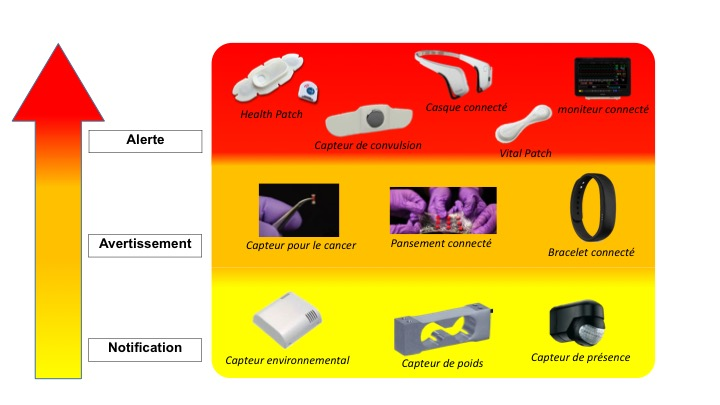
\includegraphics[width=1.4\textwidth]{alerte.jpg}
	\caption{Hiérarchisation des Signaux de Dysfonctionnement en fonction des Dispositifs}
	\label{alerte}
\end{figure}


\subsection{Prise en compte de ces problématiques dans le middleware}
 
La fiabilité d’un middleware est une exigence essentielle. Un middleware doit rester opérationnel pendant toute la durée d’une mission, même en présence de pannes. La fiabilité du middleware fait partie intégrante de la réalisation de la fiabilité au niveau du système. Chaque composant ou service dans un middleware doit être fiable pour atteindre la fiabilité globale, ce qui inclut celles de la communication, des données, des technologies et des dispositifs de toutes les couches. Les signes vitaux qui sont surveillés imposent au middleware d’être capable de transmettre les données de façon fiable sans corruption de celles-ci, à cause des données qui sont surveillées.

En cas de défaillance de notre système, le temps de récupération et la fréquence de défaillance de celui-ci sont suffisamment petits pour obtenir la disponibilité souhaitée. Les exigences en matière de fiabilité et de disponibilité doivent travailler ensemble pour assurer la plus haute tolérance aux pannes nécessaire depuis une application. Les middlewares de notre système peuvent détecter si l’un de nos capteurs est en panne, et pour cela, il va faire des requêtes à intervalles réguliers des signes vitaux, et en cas d’absence de réponse pendant un temps prédéfini, une alerte sera envoyée au personnel médical pour vérifier l’origine de l’erreur. Dans le domaine de la santé, ou la vie des patients est en jeu, nous ne pouvons pas nous permettre de laisser le patient sans surveillance médicale.

Un module de détection des pannes est présent dans les différents middlewares. En effet, de par l’importance des données fournies par ces capteurs, il faut les remplacer dès le premier indice de dysfonctionnement. De manière générale, il est important de garantir une bonne disponibilité ainsi qu’une certaine fiabilité. Ces considérations sur la détection de pannes imposent de disposer d’un module d’émission d’évènements afin que le middleware du moniteur intelligent puisse avertir immédiatement la Smart Gateway d’un dysfonctionnement d’un capteur, ou d’une valeur anormale par rapport au profil du patient (par exemple une crise cardiaque).

\subsection{Prise en compte vis-à-vis des applications}
 
Les applications que nous proposons ont pour but d’être utilisées sur des téléphones intelligents, des tablettes ou des ordinateurs. Dans le cadre de notre architecture, les applications sur lesquelles la QoS est importante sont celles liées au personnel médical.

Nous avons décrit différents processus pour assurer un minimum de QoS dans les couches précédentes, nous allons nous intéresser maintenant à comment les données vont être récupérées et utilisées. Dans ce qui a été décrit au niveau des applications, celles-ci nous permettent de centraliser les différentes données des différents capteurs. Ces données peuvent être récupérées directement à partir des capteurs ou depuis le système de stockage pour la consultation d’historique.

Les détections d’anomalies sont mises en place au niveau du Gateway et qui font remonter à l’application les différentes pannes détectées. Les applications vont pouvoir agir sur les seuils de détections d’anomalies pour que le personnel médical puisse ajuster en fonction du profil du patient les différents capteurs. Les applications utilisées par le personnel médical vont principalement être utilisées pour avertir le personnel médical de différentes alertes et anomalies provenant des différents dispositifs. Au niveau de l’application utilisée pour la consultation plus détaillée d’un profil d’un patient, l’utilisateur sera notifié des différentes alertes qui lui sont destinées pour qu’il puisse les prendre en charge avec la possibilité d’informer le système de sa non-disponibilité. Les différentes alertes vont être aussi affichées sur l’application centrale, pour une redondance des informations et pour que l’alerte soit au moins visible par l’équipe médical d’astreinte en cas de défaillance d’un dispositif d’un membre du personnel médical.

La détection des pannes matérielles se fera au niveau du middleware et de la smart Gateway qui feront remonter l’information au niveau de l’application centrale pour qu’un membre du personnel médical puisse se diriger sur la zone de la panne et prendre les mesures adéquates.

Au niveau de la disponibilité des données, le système de stockage interne à l’hôpital va permettre aux différentes applications de chercher les informations dans le réseau local et de ne pas être dépendant d’Internet.  Ce qui rendra disponible les différentes données en tout temps sauf en cas de rupture complet du réseau interne, qui est un cas qui devra être relativement rare.

Enfin la fiabilité des données qui transitent dans notre réseau va essentiellement reposer sur la fiabilité des dispositifs qui vont être présents dans notre système. Ces dispositifs seront choisis en fonction de la réputation du constructeur et de la qualité des capteurs. Outre des problèmes au niveau des capteurs, notre réseau ne devrait pas, avec les mesures de sécurité proposées, altérer les données transmises par les capteurs.      

\section{Conclusion}
TODO nouvelle conclusion
%-------------------- ancienne conclusion --------------------
%-------------------------------------------------------------
%Dans le premier rapport, nous avions présenté notre solution IoT orientée Smart Health, afin de résoudre le problème de congestion des hôpitaux dans les services de soins intensifs. Plus précisément, nous avions proposé les dispositifs et les protocoles de communication et de réseau de notre solution. Enfin, nous avions abordé les enjeux liès à la QoS, et à la sécurité et la privacité de notre solution.
%\\

%Le présent rapport a permis quant à lui de présenter le rôle du middleware dans la réponse aux problématiques de congestion de l'hôpital dans les services de soins intensifs (donc dans le cadre de notre solution). Les exigences de ces dernières ont été séparées en trois catégories, à savoir les exigences fonctionnelles, non-fonctionnelles et architecturales. Afin de remplir les différentes fonctionnalités attendues du système, différents modules au sein de notre middleware ont ainsi été identifiés. Chaque module serait destiné à remplir une fonctionnalité majeure, et à respecter une ou possiblement plusieurs exigences du middleware. Par ailleurs, nous avons présenté une conception répartie pour le middleware, conception qui peut se résumer par la présence de middlewares distincts au niveau du moniteur et de la passerelle (gateway). Nous proposons des middlewares qui pourraient opérer de manière locale comme dans un hôpital, mais qui pourraient aussi être intégrés à une plateforme IoT \cite{IBM}.

%Dans ce rapport, nous avons également mis l'accent sur les considérations sécuritaires et de confidentialité, à prendre en compte lors de la conception d'un tel système, ou plus précisément d'un tel middleware.
%\\

%L'objet du prochain rapport sera d'établir et de conceptualiser l'architecture de notre solution IoT orientée Smart Health,
%incluant la manière de stocker les données dans le Cloud, et les différentes façon dont notre solution sera exploitable à travers
%une application. Ce dernier rapport résumera la conception générale de notre solution.
%-------------------- Fin ancienne conclusion --------------------
%-----------------------------------------------------------------




\bibliographystyle{unsrt}




\bibliography{references}




\end{document}
